\documentclass[12pt,hyperref,a4paper,UTF8]{ctexart}
\usepackage{HDUReport}
\usepackage{listings}
\usepackage{xcolor}
\usepackage{graphicx}
\usepackage{setspace}
\usepackage{float}
\setstretch{1.5} % 设置全局行距为1.5倍

\usepackage{enumitem} % 载入enumitem包以便自定义列表环境
\setlist[itemize]{itemsep=0pt, parsep=0pt} % 设置itemize环境的项目间距和段落间距

\setmainfont{Times New Roman} % 英文正文为Times New Roman


\usepackage{tikz}
\usetikzlibrary{shapes.geometric, arrows}
\usetikzlibrary{positioning, arrows.meta}
\usetikzlibrary{calc}
%封面页设置
{   
    %标题
    \title{ 
        \vspace{1cm}
        \heiti \Huge \textbf{《单片机原理及应用》作业报告} \par
        \vspace{1cm} 
        \heiti \Large {\underline{实验报告4第三部分:24秒倒计时}   } 
        \vspace{3cm}
    
    }

    \author{
        \vspace{0.5cm}
        \kaishu\Large 学院\ \dlmu[9cm]{卓越学院} \\ %学院
        \vspace{0.5cm}
        \kaishu\Large 学号\ \dlmu[9cm]{23040447} \\ %班级
        \vspace{0.5cm}
        \kaishu\Large 姓名\ \dlmu[9cm]{陈文轩} \qquad  \\ %学号
        \vspace{0.5cm}
        \kaishu\Large 专业\ \dlmu[9cm]{智能硬件与系统(电子信息工程)} \qquad \\ %姓名 
    }
        
    \date{\today} % 默认为今天的日期,可以注释掉不显示日期
}
%%------------------------document环境开始------------------------%%
\begin{document}

%%-----------------------封面--------------------%%
\cover
\thispagestyle{empty} % 首页不显示页码
%%------------------摘要-------------%%
%\newpage
%\begin{abstract}




%\end{abstract}

%\thispagestyle{empty} % 首页不显示页码

%%--------------------------目录页------------------------%%
% \newpage
% \tableofcontents
% \thispagestyle{empty} % 目录不显示页码

%%------------------------正文页从这里开始-------------------%
\newpage
\setcounter{page}{1} % 让页码从正文开始编号

%%可选择这里也放一个标题
%\begin{center}
%    \title{ \Huge \textbf{{标题}}}
%\end{center}


\textbf{设计实现24秒计时器。要求:
(1)倒计时功能
(2)24秒复位键功能
(3)启动/暂停键功能}


\section{实验代码}

\begin{lstlisting}[language=C, caption={实验程序}]
#include <reg51.h> // 单片机头文件

unsigned char code Tab[] = {0xC0, 0xF9, 0xA4, 0xB0, 0x99, 0x92, 0x82, 0xF8, 0x80, 0x90}; // 共阳数码管码段表
unsigned char Dat[] = {0, 0, 2, 4}; // 初始时间为24秒
int Dat_int=24;
int i; // 定义变量,作为循环
unsigned char tmp; // 定义片选变量
unsigned char KeyState = 0x0F; // 按键状态变量,初始值为高电平(未按下)
bit isRunning = 1; // 计时器运行状态标志位

#define KEY1 (P1 & 0x01) // 按键1连接到 P1.0
#define KEY2 (P1 & 0x02) // 按键2连接到 P1.1
#define KEY3 (P1 & 0x04) // 按键3连接到 P1.2
#define KEY4 (P1 & 0x08) // 按键4连接到 P1.3
#define TIM_SET 24 //此程序设置几秒定时 方便调试

void Delay() // 延时子程序,作为数码管显示延迟
{
    unsigned char i;
    for (i = 0; i < 100; i++);
}

void Timer1_Init() // 定时器1初始化
{
    TMOD |= 0x10; // 设置定时器1为模式1(16位定时器)
    TH1 = 0x00;   // 定时器初值高字节(1秒定时)
    TL1 = 0x00;   // 定时器初值低字节
    ET1 = 1;      // 使能定时器1中断
    EA = 1;       // 使能总中断
    TR1 = 1;      // 启动定时器1
}

void Timer1_ISR() interrupt 3 // 定时器1中断服务函数
{
    static int counter=0;
    TH1 = 0x3C;   // 重装定时器初值高字节
    TL1 = 0xAF;   // 重装定时器初值低字节 (15535)D=(3CAF)H 即65535-50000=15535 延时50ms;

    counter++;
    if (counter==20) //50*20=1000ms 1s定时器中断
    {
        counter=0;
        Dat_int--;
        if (Dat_int<0)
        {
            Dat_int=TIM_SET;
        }
        Dat[2]=Dat_int/10;
        Dat[3]=Dat_int%10;
    }
}

void Ext0_Init() // 外部中断0初始化
{
    IT0 = 1; // 设置外部中断0为下降沿触发
    EX0 = 1; // 使能外部中断0
    EA = 1;  // 使能总中断
}

void Ext0_ISR() interrupt 0 // 外部中断0服务函数 正常工作
{ 
   //进入中断后,说明有按键按下,再进行扫描,这样大大节省程序运行资源
		Delay(); //延时消抖
		if (KEY1==0) //按键1 p1.0按下 实现复位
		{
			Dat_int=0;
		}
		if (KEY2==0)
		{
			TR1=(TR1==1)?0:1; //切换TR1状态 控制定时器1开启与否
		}
	 
}

void main()
{
    Timer1_Init(); // 初始化定时器1
    Ext0_Init();   // 初始化外部中断0
	
    Dat[2]=TIM_SET/10; 
    Dat[3]=TIM_SET%10; //按照宏定义初始化Dat(数码管显示直接控制数组)
    Dat_int=TIM_SET;
	
	
    while (1) // 无限循环 数码管扫描主进程
    {
        tmp = 0x01; // 片选初值
        for (i = 0; i < 4; i++) // 循环4次
        {
            P2 = tmp; // 片选初值
            P0 = Tab[Dat[i]]; // 输出某一位数字的码段值
            tmp = tmp << 1; // 片选值左移一位
            Delay(); // 调用延时
        }
    }
}
\end{lstlisting}

\section{实验效果}

\begin{figure}[H] % [H] 表示强制当前位置插入
    \centering
    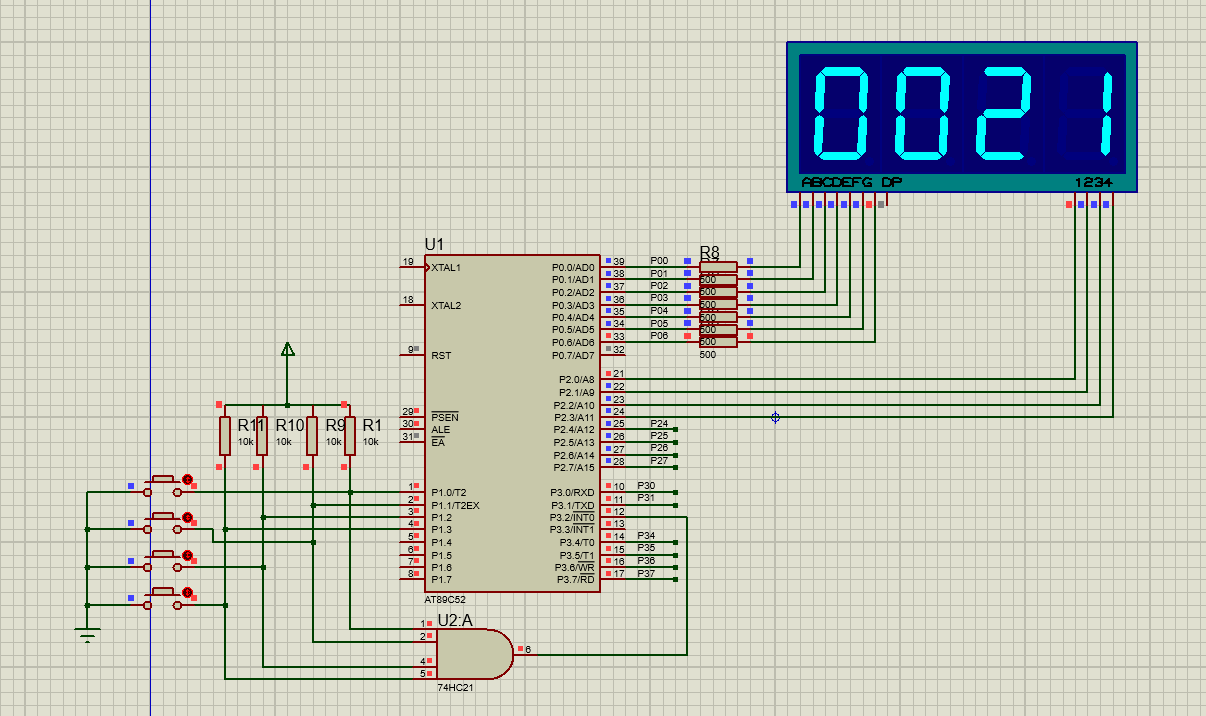
\includegraphics[width=0.9\textwidth]{figures/201.png} % 调整宽度为文本宽度的 80%
    \caption{正常计时:显示到21 } %图片标题
    \label{fig:example} % 图片标签,用于引用
\end{figure}

\begin{figure}[H] % [H] 表示强制当前位置插入
    \centering
    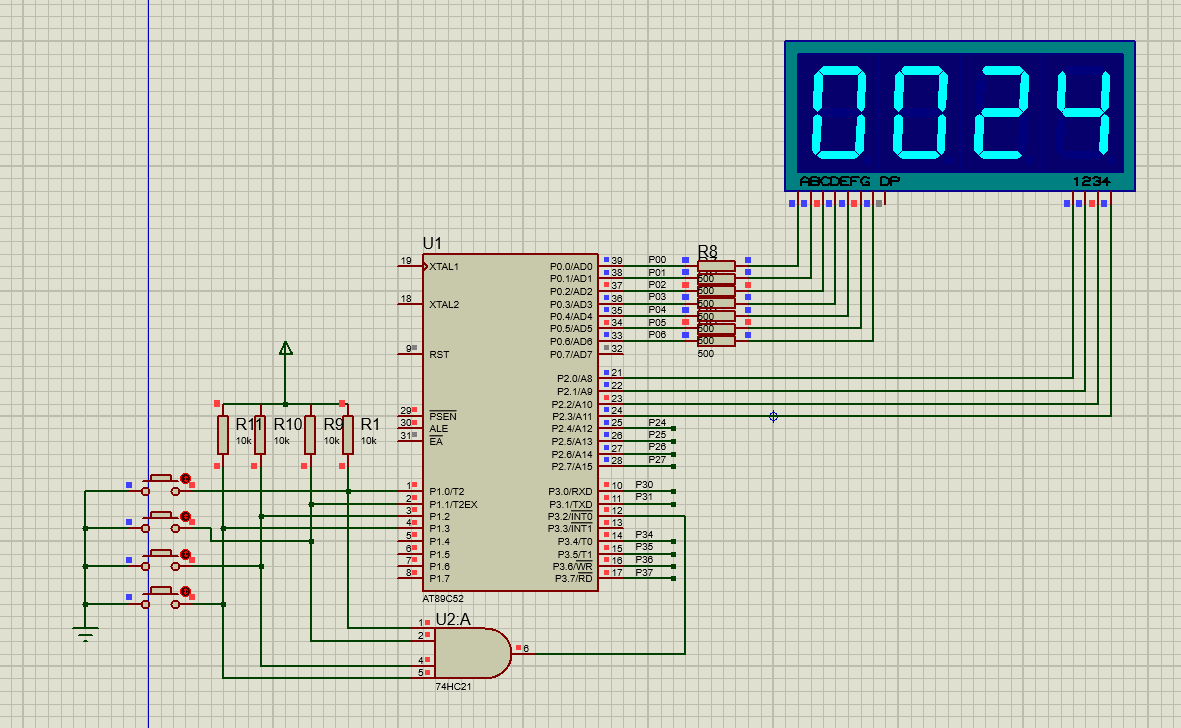
\includegraphics[width=0.9\textwidth]{figures/202.png} % 调整宽度为文本宽度的 80%
    \caption{复位至24} %图片标题
    \label{fig:example} % 图片标签,用于引用
\end{figure}

\begin{figure}[H] % [H] 表示强制当前位置插入
    \centering
    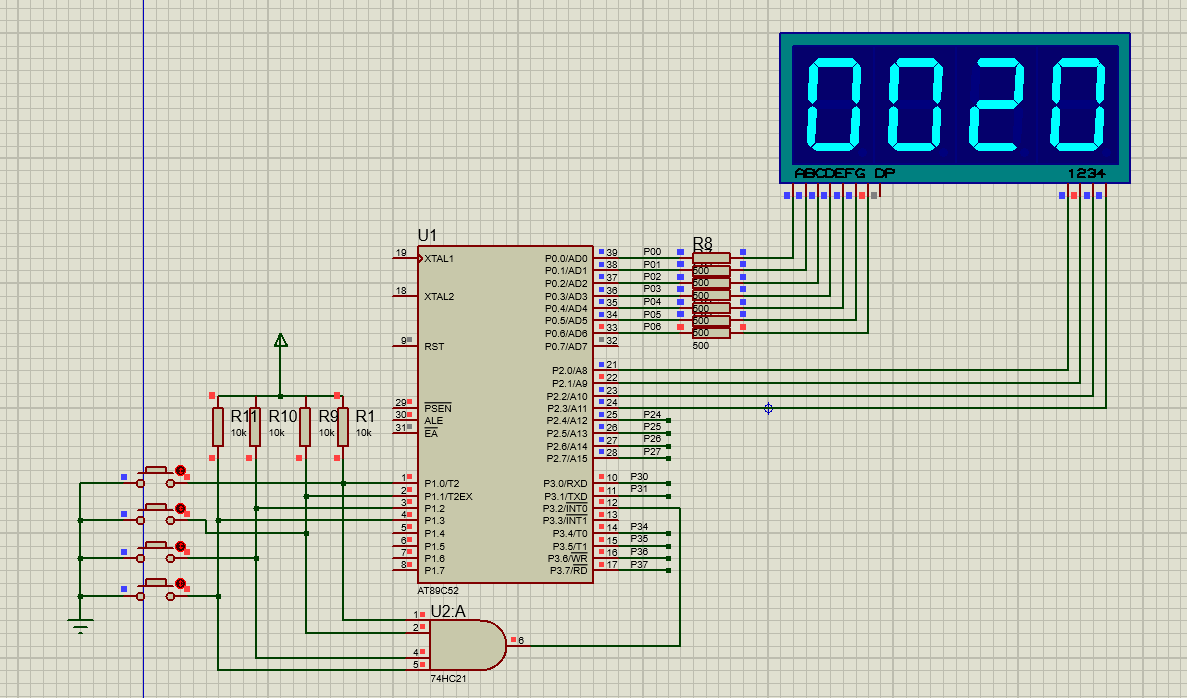
\includegraphics[width=0.9\textwidth]{figures/203.png} % 调整宽度为文本宽度的 80%
    \caption{暂停在20 } %图片标题
    \label{fig:example} % 图片标签,用于引用
\end{figure}


\section{流程图}


\begin{figure}[H] % [H] 表示强制当前位置插入
        \centering
        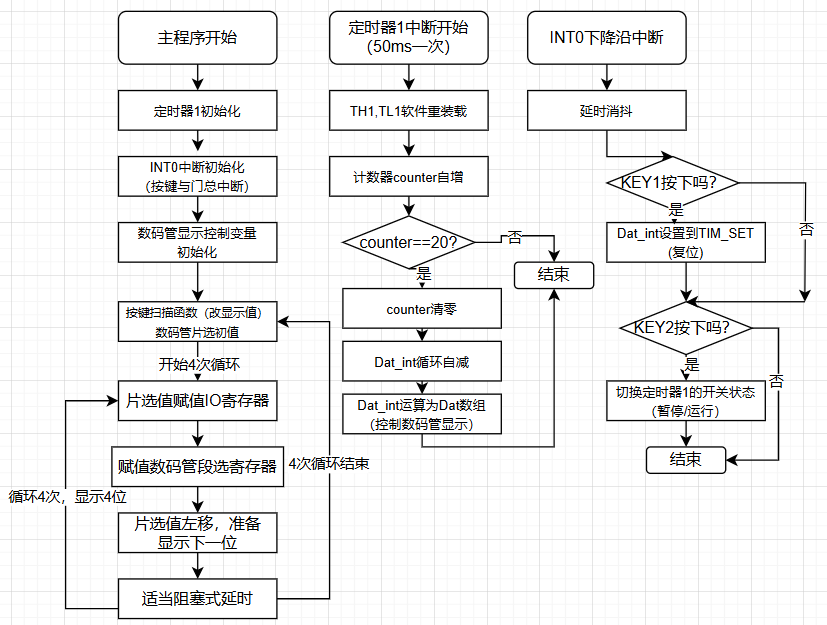
\includegraphics[width=1\textwidth]{figures/301.png} % 调整宽度为文本宽度的 80%
        \caption{系统控制流程图} %图片标题
        \label{fig:example} % 图片标签,用于引用
\end{figure}



\section{实验体会}


本实验通过动态扫描方式结合四输入与门的中断控制,实现按键的中断触发扫描,以此作为按键实现相应功能之基础;结合定时器溢出中断,实现定时显示值自减;
在迁移已有的数码管主线程显示,实现系统的整体功能;同时也发现定时不一定准确(需要调参),暂停时复位无相应及时显示等问题,需要做出一定改进。




\end{document}